% !TEX program = xelatex

\documentclass{beamer}
\usepackage[utf8]{inputenc}
\usepackage{listings}
\usepackage{fontspec} % 定制字体
\usepackage{xeCJK}
\usepackage{utopia} %font utopia imported
%\usepackage[UTF8,noindent]{ctexcap}
\usepackage{latexsym,amssymb,amsmath,amsbsy,amsopn,amstext,xcolor,multicol}
\usepackage{graphicx,wrapfig,fancybox}
\usepackage{booktabs}
% \usetheme{Rochester}
\usetheme{Madrid}
\usecolortheme{default}
 % 衬线字体:Linux Libertine
    % BoldFont 可以选择 Bold 字重或者 Semibold 字重
    % BoldItalicFont 也有对应 BoldFont 的字重选择
    % 这里使用 Semibold 字重
    \setmainfont{LinLibertine_R.otf}[
      BoldFont = LinLibertine_RZ.otf,
      ItalicFont = LinLibertine_RI.otf,
      BoldItalicFont = LinLibertine_RZI.otf]
  % % 无衬线字体:Linux Biolinum
  % \setsansfont{LinBiolinum_R.otf}
      %   [BoldFont = LinBiolinum_RB.otf,
      % ItalicFont = LinBiolinum_RI.otf,
      % BoldItalicFont = LinBiolinum_RBO.otf]
  % % 等宽/打印机字体:Linux Libertine Mono
  % \setmonofont{LinLibertine_M.otf}[
  %     BoldFont = LinLibertine_MB.otf,
  %     ItalicFont = LinLibertine_MO.otf,
  %     BoldItalicFont  = LinLibertine_MBO.otf]
  % \setCJKmainfont[ItalicFont={AR PL UKai CN},
  % BoldFont={WenQuanYi Micro Hei}]{IPAMinCho,IPA明朝}
  
  % \setsansfont{Helvetica}
  \setCJKsansfont{WenQuanYi Micro Hei}
  \setCJKmonofont{WenQuanYi Micro Hei Mono}

  \newfontfamily\menlo{WenQuanYi Micro Hei Mono}
  \usepackage{xcolor} % 定制颜色
  \definecolor{mygreen}{rgb}{0,0.6,0}
  \definecolor{mygray}{rgb}{0.5,0.5,0.5}
  \definecolor{mymauve}{rgb}{0.58,0,0.82}
  \lstset{ %
  backgroundcolor=\color{white},      % choose the background color
  basicstyle=\footnotesize\ttfamily,  % size of fonts used for the code
  columns=fullflexible,
  tabsize=4,
  breaklines=true,               % automatic line breaking only at whitespace
  captionpos=b,                  % sets the caption-position to bottom
  commentstyle=\color{mygreen},  % comment style
  escapeinside={\%*}{*)},        % if you want to add LaTeX within your code
  keywordstyle=\color{blue},     % keyword style
  stringstyle=\color{mymauve}\ttfamily,  % string literal style
  frame=single,
  rulesepcolor=\color{red!20!green!20!blue!20},
  % identifierstyle=\color{red},
  language=c++,
  }
  \renewcommand{\thefootnote}{\fnsymbol{footnote}} %*, **, ***
  % \let\thefootnote\relax\footnotetext{Footnotetext without footnote mark}
  %------------------------------------------------------------
%This block of code defines the information to appear in the
%Title page
\title[毕设答辩] %optional
{基于解析数据的DNS安全评估与增强}
\subtitle{毕设答辩}


\author[芦迪] % (optional)
{无41 芦迪}

\institute[THU, EE] % (optional)
{
  \normalsize{指导老师:李星} \\
  \
  
  Department of Electronic Engineering,\\
  Tsinghua University
  
}

\date[2018.6.15] % (optional)
{June 15, 2018}

\logo{
\includegraphics[height=1.5cm]{images/thuee-logo.png}}

%End of title page configuration block
%------------------------------------------------------------



%------------------------------------------------------------
%The next block of commands puts the table of contents at the 
%beginning of each section and highlights the current section:

\AtBeginSection[]
{
  \begin{frame}
    \frametitle{目录}
    \tableofcontents[currentsection]
  \end{frame}
}
%------------------------------------------------------------


\begin{document}
%The next statement creates the title page.
\frame{\titlepage}


%---------------------------------------------------------
%This block of code is for the table of contents after
%the title page
\begin{frame}
\frametitle{目录}
\tableofcontents
\end{frame}
%---------------------------------------------------------
\section{背景介绍}
\begin{frame}{DNS}
  \textbf{DNS}: Domain Name System,域名系统
  \begin{itemize}
    \item 域名(www.tsinghua.edu.cn) \(\Longleftrightarrow\) IP地址(166.111.4.100)
    \item 重要的互联网基础设施,遭到攻击损失无法估量
    \begin{figure}
      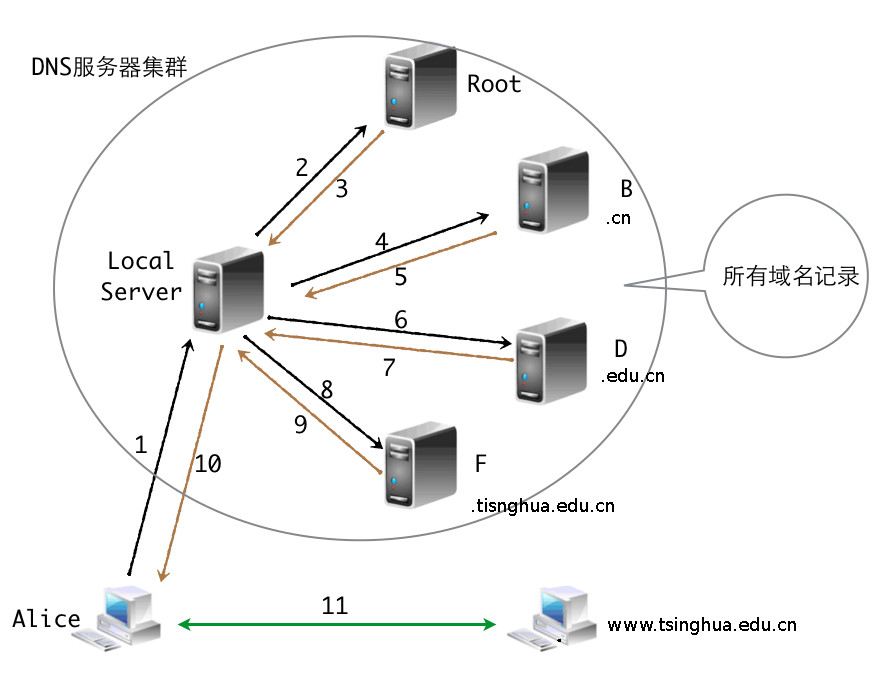
\includegraphics[height=5cm]{figures/dns/name_resolution.jpg}
      \end{figure}
    
   
  \end{itemize}
  
\end{frame}

\begin{frame}{DNS攻击}
  \begin{itemize}
    \item DNS 易受攻击
      \begin{itemize}
        \item 协议脆弱性:UDP、明文
        \item 系统脆弱性:Open Resolvers、路径复杂
        \item 常见攻击类型
        \begin{itemize}
          \item DNS 劫持:将DNS请求定向到非法解析器
          \item DNS 缓存中毒:将虚假域名数据注入到缓存中
        \end{itemize}
        \item DNS攻击实例:
        \begin{itemize}
          \item 2014年1月21日下午,大陆境内发生了严重的DNS故障,所有的通用顶级域(.com/.net/.org等)遭到DNS劫持/污染,所有域名被指向到一个位于美国的IP地址(65.49.2.178)
          \item  2016 年 10 月21日,网络提供商 Dynamic Network Service的域名服务器遭遇DDoS 攻击,美国一个很大区域内的互联网在十个小时内无法访问Twitter、Ebay、Netflix、Amazon、Paypal 等网站
          \item ......
        \end{itemize}    
      \end{itemize}
  \end{itemize}
\end{frame}

% \begin{frame}{概念说明}
%   DNS,Resolver,DNSSEC,IPv6,证书
% \end{frame}

\begin{frame}{CDN与负载均衡}
  \begin{itemize}
    \item 因为CDN与负载均衡的普遍存在,域名解析情况更加复杂
    \begin{itemize}
    \item CDN:Content Delivery Network
    \begin{itemize}
      \item 部署边缘服务器,使用户就近获取所需内容,降低网络拥塞
    \end{itemize}
    \begin{figure}
    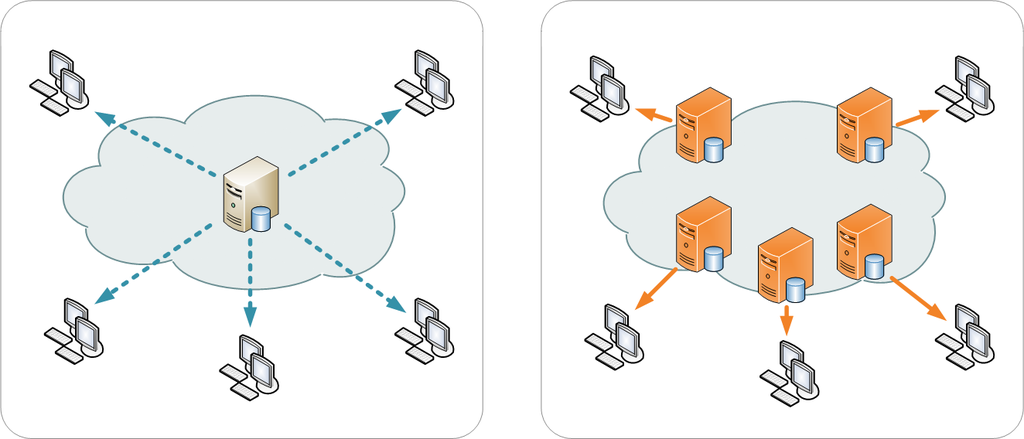
\includegraphics[height=3cm,width=7.07cm]{images/NCDNCDN.png}
    \end{figure}
    
    \item 负载均衡:在多个服务器中分配负载,最优化资源使用,避免过载
    \end{itemize}
    \item 一个域名会解析出多个IP,一个IP也可以对应多个域名
  \end{itemize}

\end{frame}
\begin{frame}{网络安全增强}
  互联网天然缺乏安全性,通过完善协议可以增强安全性
  \begin{itemize}
    \item DNSSEC:DNS安全扩展
    \begin{itemize}
      \item 使用公钥密码机制,以DNS资源记录计算数字签名,验证数字签名确保解析结果真实
      \item 提供数据来源、数据完整性和否定存在验证
    \end{itemize}
    \item IPv6:下一代互联网协议
    \begin{itemize}
      \item IPv6内嵌IPSec协议族的AH和ESP,从协议上提升安全性
      \item IPv6地址空间大,增大扫描难度,可减缓现有攻击
    \end{itemize}
    \item DNS over HTTPS
    \begin{itemize}
      \item 使用HTTPS传输解析信息,增强了客户端和递归解析器之间的隐私和安全性
    \end{itemize}
  \end{itemize}  
\end{frame}
\begin{frame}{前人工作}
  目前在对DNS数据进行测量、分析的领域内已经有很多的研究成果。
  \begin{itemize}
    
    \item 文献 \cite{Kuhrer2015}\footnote[1]{Going Wild: Large-Scale Classification of Open DNS Resolvers} 通过对DNS解析结果进行过滤,并对HTTP请求返回的内容进行聚类,系统地分析了非合法的DNS响应
    \item 文献\cite{Scott2016}\footnote[2]{Joint Analysis of CDNs and Network-Level Interference using Satellite} 利用开放解析器通过采集 DNS 解析数据来识别 CDN 的部署与解析中存在的网络干扰
    \item 文献\cite{Pearce2017}\footnote[3]{Global Measurement of DNS Manipulation}采用一致性和独立的可验证性指标,通过对解析结果IP地址、自治域、HTTP内容、HTTPS证书等内容进行验证,实现了对网络审查的检测
    \item 还有其他文献对测量什么、如何测量、确定异常行为等方面进行了深入的研究
  \end{itemize}
\end{frame}
\begin{frame}{毕设内容}
  \begin{itemize}
    \item 对权威服务器记录内容进行考察
    \begin{itemize}
      \item 分析域名解析数据,了解域名或解析器对IPv6、DNSSEC、HTTPS的支持情况,评估安全现状
      \begin{itemize}
        \item 根据A记录与AAAA记录,判断IPv6支持情况  
        \item 根据RRSIG记录,判断DNSSEC支持情况
        \item 测试(域名, IP地址),判断HTTPS支持情况
      \end{itemize}
    \end{itemize}
    \item 对开放递归服务器进行考察
    \begin{itemize}
      \item Open Resolvers 基本情况
      \item 对DNS解析返回的IP地址进行判别与分类
      \begin{itemize}
        \item 结果正常:CDN?负载均衡?
        \item 结果有误:DNS劫持?缓存中毒?
      \end{itemize}
    \end{itemize}
  \end{itemize}
  
\end{frame}




\section{系统设计与实施}
\subsection{整体架构}
\begin{frame}{系统设计}

  \begin{figure}
    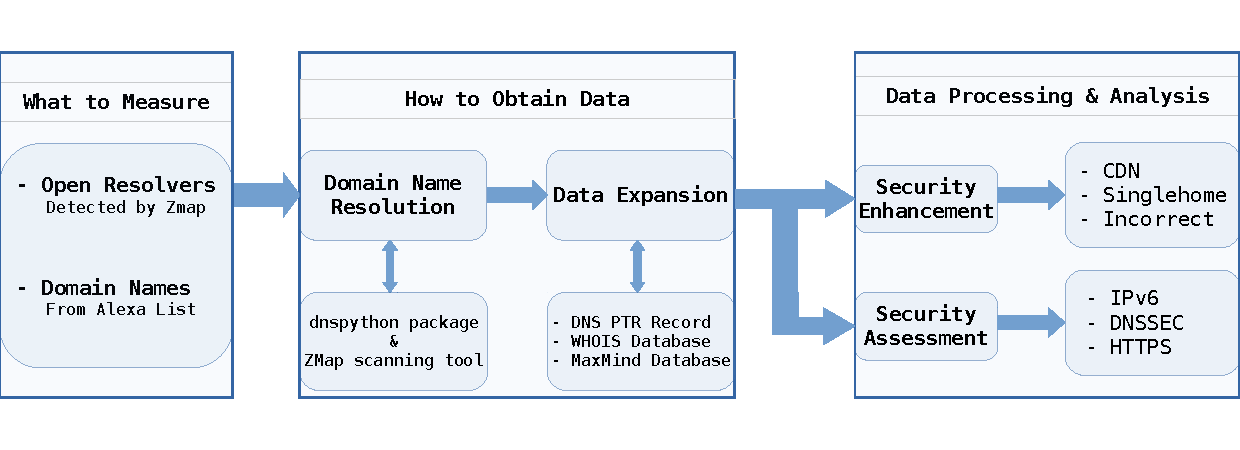
\includegraphics[height=4cm]{figures/sysoverview.pdf}
    \caption{整体系统设计}
  \end{figure}
\end{frame}
\subsection{测量内容}

\begin{frame}{测量什么}
  \begin{itemize}
    \item 对开放解析器状况进行评估:ZMAP扫描IPv4 空间,设置过滤条件,获得包含1.6万开放解析器的集合
    \begin{itemize}
      \item 设置过滤条件:响应时间在 3 秒内、PTR 反向查询可获得结果......
      \item 使用ZMap进行扫描
      \begin{itemize}
        \item 对IPv4网络空间进行快速测量的工具
          \item 对单端口大规模测量有着很好的支持
          \item 不记录状态,可在45min扫描整个IPv4空间
          \item 支持TCP SYN 、UDP等多种扫描模式
      \end{itemize}
    \end{itemize}

  \end{itemize}

\end{frame}



\begin{frame}{测量什么}
  \begin{itemize}
    \item 对开放解析器状况进行评估:ZMAP扫描IPv4 空间,设置过滤条件,获得包含1.6万开放解析器的集合
    \item 对域名安全状况进行评估:选择Alexa统计的全球访问量前10000的网站 × 手动选择的包含40个开放解析器的集合
    \begin{columns}
      
      \begin{column}{0.5\textwidth}
        
        \begin{table}
          \tiny
        \begin{tabular}{r|l}
          \toprule
          Num. & Domain Name\\
          \midrule
          1&google.com\\
          2&youtube.com\\
          3&facebook.com\\
          4&baidu.com\\
          5&wikipedia.org\\
          6&yahoo.com\\
          7&reddit.com\\
          8&google.co.in\\
          ......&...... \\
          \bottomrule
          \end{tabular}
          \caption{\scriptsize{Top Domain Names}}
        \end{table}
      \end{column}
      \begin{column}{0.5\textwidth}
        \begin{table}
          \tiny
        \begin{tabular}{r|l|l}
          \toprule
          Resolver& Owner&DNSSEC\\
          \midrule
          8.8.8.8 & Google&Y \\
          4.2.2.2&     MicroSoft&Y \\
          9.9.9.9&  IBM&Y \\
          8.26.56.26& Comodo&Y \\
          180.76.76.76&Baidu&Y\\
          202.141.162.123&USTC&Y\\
          223.6.6.6&Ali&N \\
          114.114.114.114 & 114DNS&N \\
          ......&...... &......\\
          \bottomrule
          \end{tabular}
          \caption{\scriptsize{Open Resolvers}}
        \end{table}
      \end{column}
      \end{columns}
  \end{itemize}

\end{frame}

\begin{frame}{测量什么}
  \begin{itemize}
    \item 对开放解析器状况进行评估:ZMAP扫描IPv4 空间,设置过滤条件,获得开放解析器的集合
    \item 对域名安全状况进行评估:选择Alexa统计的全球访问量前10000的网站 × 手动选择的包含少量开放解析器的集合
    \item 对 DNS 查询结果进行分类:Alexa Top 1000 × 扫描获得的开放解析器列表
  \end{itemize}

\end{frame}

\subsection{数据获取}

\begin{frame}{获取数据}
  \begin{itemize}
    \item dnspython进行多样化查询
    \begin{itemize}
      \item Python的一个强大的DNS工具包
      \begin{itemize}
        \item 采用多种模式进行DNS查询的操作
        \item 对收到的DNS响应进行解析
      \end{itemize}
      \item DNSSEC 查询、A记录查询、AAAA记录查询、基于tcp的查询
      \item 单线程因网络延迟导致低效率\(\Rightarrow\)多线程,维护查询线程池
    \end{itemize}
    \item ZMap进行快速DNS查询
    \begin{itemize}
      \item 可以快速进行大量DNS查询
      \item 以Open Resolvers为白名单,构建DNS请求包并发送
      \item 解析回包并保存
    \end{itemize}

  \end{itemize}
  例:

  \fbox{zmap -M udp -p 53 –probe-args=file:tsinghua.edu.cn.pkt -N 100}
\end{frame}

\begin{frame}{数据扩充}
  采用多种方式对数据进行扩充,便于之后的处理:
  \begin{itemize}
    \item DNS PTR Record
    \begin{itemize}
      \item PTR 记录包含在 “in-addr.arpa”这一域名下
      \item 通常由控制这个 IP 的组织进行维护
      \item 对属于已知服务的 IP 通常提供规范的名称
    \end{itemize}
    \item WHOIS Database
    \begin{itemize}
      \item 包含 IP 地址的所有权信息
    \end{itemize}
    \item MaxMind Database
    \begin{itemize}
      \item 获取 IP 地址的地理位置信息
    \end{itemize}
    \item BGP 路由表数据
    \begin{itemize}
      \item IP 地址的AS编号
    \end{itemize}
  \end{itemize}
  
\end{frame}

\subsection{安全评估与增强}
\begin{frame}{安全评估}
  
  \begin{itemize}
    \item 通过DNS查询可以了解IPv6、DNSSEC等协议部署情况
    \begin{enumerate}
      \item 根据A记录与AAAA记录,判断IPv6支持情况
      \begin{figure}
        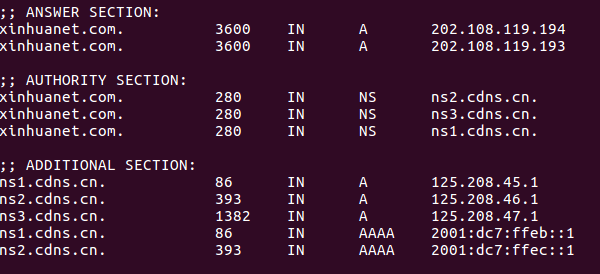
\includegraphics[height=2.74cm,width=6cm]{images/aaaa.png}
      \end{figure} 
  
      \item 根据RRSIG记录,判断DNSSEC支持情况
      \begin{figure}
        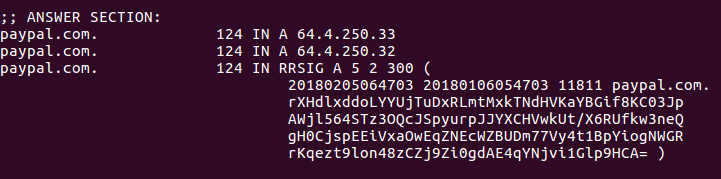
\includegraphics[height=1.79cm,width=7.21cm]{images/dnssec.png}
      \end{figure} 
    \end{enumerate}
  \end{itemize}
\end{frame}

\begin{frame}{安全评估}
  \begin{itemize}
    \item HTTPS部署情况及正确性
    \begin{itemize}
      \item 使用数字证书来验证站点的身份,加密用户和站点之间的数据交换
      \item 对于解析到的IP地址,对其 443 端口发起连接请求,验证是否支持HTTPS
      \item 对于支持HTTPS的IP地址,对其证书进行验证,将验证通过的(domain, ip, resolver)对标记为正确
    \end{itemize}
    % \item DNSSEC正确性
    % \begin{itemize}
    %   \item 使用数字签名来验证 DNS 数据的完整性,从而确保用户可以到达预期的 IP 地址
    %   \item 大多数解析器支持 DNSSEC,但部署了 DNSSEC 的域名仍较少
    %   \item 通过公钥与签名验证解析记录真实性与完整性,从信任锚开始对信任链进行验证
    % \end{itemize}
  \end{itemize}

\end{frame}

\begin{frame}{安全增强}
  \begin{itemize}
    \item 通过DNS解析,由域名得到IP地址,我们将其分为以下类别:
  \begin{enumerate}
    \item 单归属域名返回唯一IP地址
    \item CDN或负载均衡返回的结果
    \item DNS劫持、缓存中毒或其他错误结果
  \end{enumerate}
  \item 对解析结果的识别流程
  \begin{enumerate}
    \item IP地址信息扩充,进行初步聚合
    \item 采用文献\cite{Scott2016}中的联合分析算法,实现对CDN与网络干扰的分别聚类
    \item HTTPS对解析到的IP地址进行验证,作为Groundtruth
  \end{enumerate}
  \end{itemize}
\end{frame}

\begin{frame}{联合聚类算法}
  \begin{itemize}
    \item 定义两个函数\texttt{DomainSimilarity}与\texttt{IPTrust}
    \begin{itemize}
      \item \texttt{DomainSimilarity}表示两个域名的相似程度
      \item \texttt{IPTrust}表示IP是域名的正确解析结果的可信度
      \item (A)中,a.com与b.com应当拥有一个高的 \texttt{DomainSimilarity},因为它们被解析到相同的IP地址上
    \item (B)中,IP地址210.211.21.90应当拥有一个低的\texttt{IPTrust},因为很多不相关的域名解析了它
    \item 给定初始值,迭代计算,直到收敛
    \end{itemize}
  \end{itemize}
  \begin{figure}[H] % use float package if you want it here
    \centering
    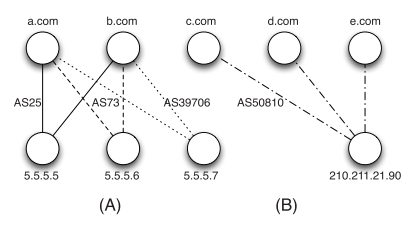
\includegraphics[width=5cm]{figures/ip_domains.png}
    % \caption{域名与IP地址}
    \label{fig:ip_domains}
  \end{figure}
  \begin{itemize}
    \item 文献\cite{Scott2016}中通过对比域名图标与IP地址图标对结果进行验证
    \item 我们通过检验HTTPS结果对结果进行验证
  \end{itemize}
\end{frame}
\subsection{实验部署}

\begin{frame}{部署与实施}
  \begin{itemize}
    \item 实验平台信息
    \begin{itemize}
      \item 实验平台:DigitalOcean 服务器
      \item 操作系统:Ubuntu 16.04
      \item 公网IP:206.189.75.45,2604:a880:2:d0::207d:a001
      \item 数据保存:MySQL, phpmyadmin
  
    \end{itemize}
    \item 数据的获取
    \begin{enumerate}
      \item ZMap对IPv4空间进行扫描并过滤,得到16488个解析器
      \item dnspython进行DNS查询操作,Alexa Top 10000 域名在一个手动选取的40个解析器的列表上进行查询,共获得365517个查询结果,802058个(domain,res,ip)三元组,74894个(domain,ip)二元组
      \item ZMap进行DNS查询操作,Alexa Top 1000 域名在16488个开放解析器上进行查询,最终获得926万个(domain, res, ip)三元组,16万(domain, ip)二元组
    \end{enumerate}
  \end{itemize}
  
\end{frame}
\section{数据分析与结论}


\subsection{对权威服务器的考察}

\begin{frame}{IPv6与DNSSEC}

  Alexa Top 10000 顶级域名分布情况:

  % \begin{figure}[htbp]
  %   \centering
  %   \begin{minipage}[htbp]{150pt}
  %     \centering
  %     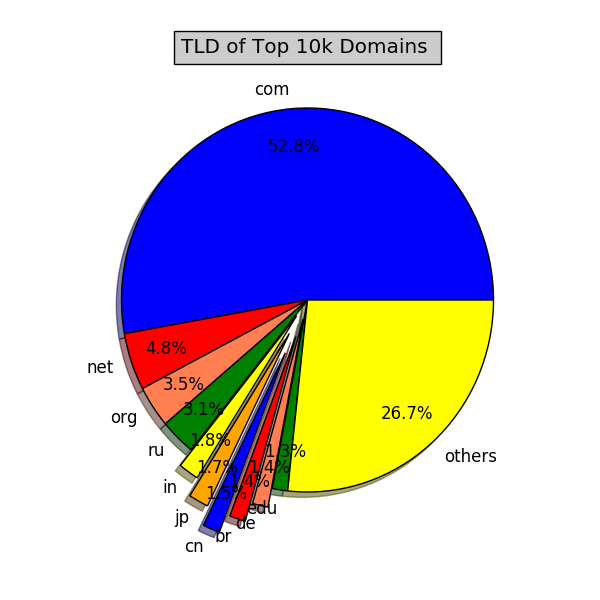
\includegraphics[width=150pt]{images/figure/figure_2.png}
  %     \caption{\scriptsize{顶级域名分布}}
  %     \label{fig:4}
  %   \end{minipage}
  %   \hspace{10pt}%
  %   \begin{minipage}[htpb]{150pt}
  %     \centering
  %     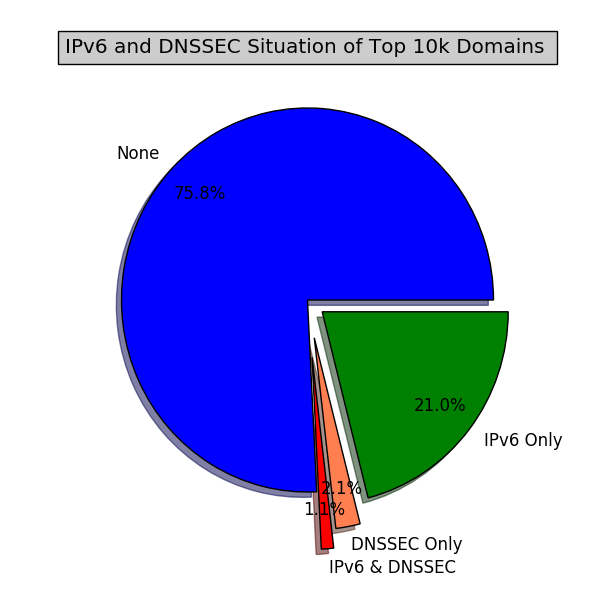
\includegraphics[width=150pt]{images/figure/figure_3.png}
  %     \caption{\scriptsize{IPv6/DNSSEC Crosscheck}}
  %     \label{fig:5}
  %   \end{minipage}
  %   \end{figure}
\begin{figure}
  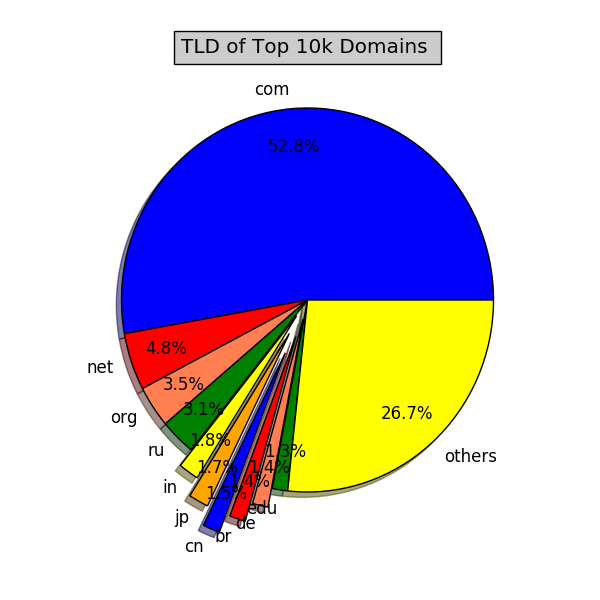
\includegraphics[height=7cm]{images/figure/figure_2.png}
\end{figure}

\end{frame}
\begin{frame}{IPv6、DNSSEC、HTTPS}

  IPv6、DNSSEC、HTTPS整体及在com、net和cn顶级域下的支持情况:

  \begin{table}
  \begin{tabular}{c|c|c|c|c}
    \toprule
           & Count & HTTPS & IPv6 & DNSSEC \\
    \midrule
    ALL & 8849& 5376,60.8\% &2159,24.4\%& 290,3.28\% \\
    com&  4744 &2874,60.6\%& 1073,22.6\% &102,2.15\% \\
    net&409  &239,58.4\%  &139,34.0\% &14,3.42\% \\
    cn&156&42,26.9\% &6,3.85\%  & 1,0.64\% \\
    \bottomrule
    \end{tabular}
  \end{table}
  从表中可以看出:
  \begin{itemize}
    \item cn顶级域名下HTTPS、IPv6、DNSSEC的支持情况都要远远低于平均
    \item net顶级域名下IPv6和DNSSEC的支持情况要高于平均
  \end{itemize}
\end{frame}



\begin{frame}{联合分布情况}
  下面我们考察HTTPS、IPv6、DNSSEC在整体及不同顶级域名下的联合分布情况,如下表所示:
  \begin{table}
    \tiny
    \begin{tabular}{c|c|c|c|c}
      \toprule
             & HTTPS+IPv6 & HTTPS+DNSSEC & IPv6+DNSSEC & IPv6+DNSSEC+HTTPS \\
      \midrule
      ALL & 1796& 201 &114& 88 \\
      com&  874 &82& 42 &38 \\
      net&120  &10&6&5 \\
      cn&2&0 &0  & 0 \\
      \bottomrule
      \end{tabular}
    \end{table}
  经过进一步的分析,我们发现:
  \begin{itemize}
    \item 在部署IPv6同时,部署HTTPS的概率很大
    \item DNSSEC 的部署情况与IPv6和HTTPS的部署情况无关
  \end{itemize}
\end{frame}

\begin{frame}{HTTPS与DNSSEC}

  \begin{figure}
    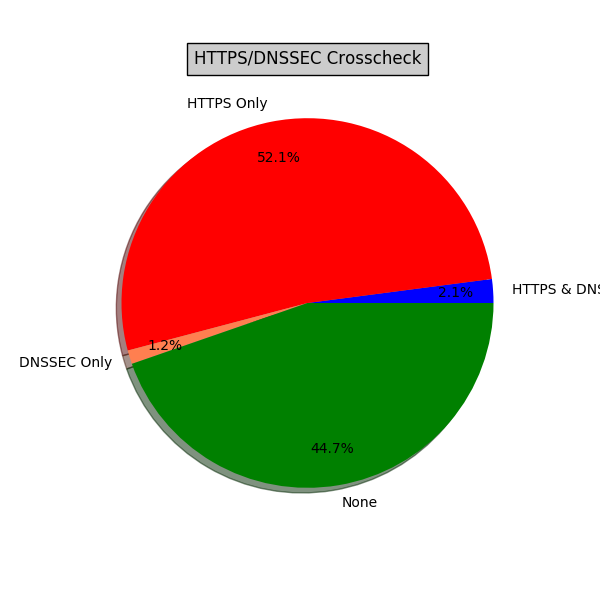
\includegraphics[height=5cm]{images/figure/httpsdnssec.png}
  \end{figure}

  \begin{itemize}
    \item 仅仅 HTTPS 验证成功或者两者都没有验证成功的结果是最常见的
    \item DNSSEC 验证通过而 HTTPS 没有完成验证的情况最令人费解
    \begin{itemize}
      \item 考察了这个类别,其中有很多成人网站、政府机构和教育机构的网站
    \end{itemize}
  \end{itemize}
  \end{frame}
  % \begin{figure}[htbp]
  %   \centering
  %   \begin{minipage}[htbp]{150pt}
  %     \centering
  %     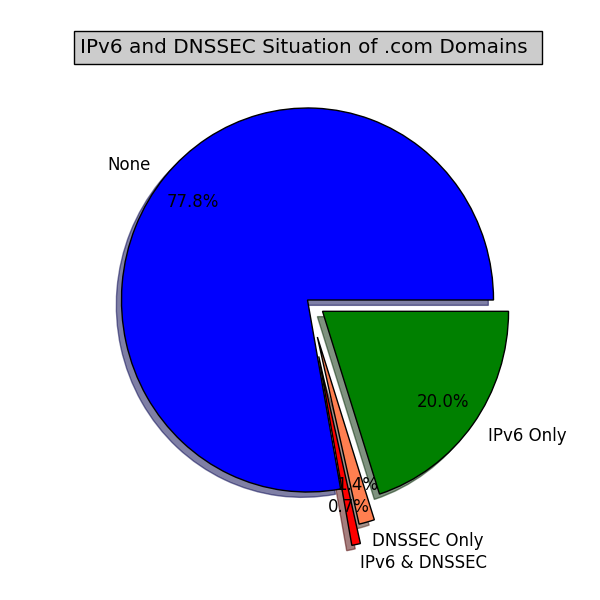
\includegraphics[width=150pt]{images/figure/figure_1.png}
  %     \caption{\scriptsize{IPv6/DNSSEC Crosscheck in .com Domain}}
  %     \label{fig:4}
  %   \end{minipage}
  %   \hspace{10pt}%
  %   \begin{minipage}[htpb]{150pt}
  %     \centering
  %     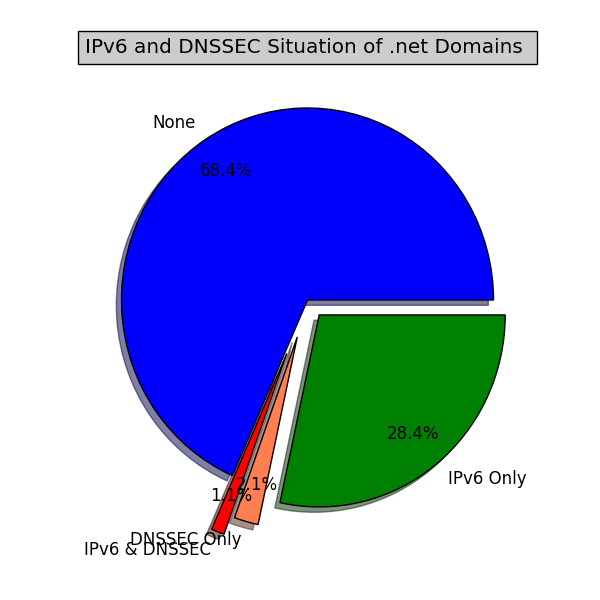
\includegraphics[width=150pt]{images/figure/figure_4.png}
  %     \caption{\scriptsize{IPv6/DNSSEC Crosscheck in .net Domain}}
  %     \label{fig:5}
  %   \end{minipage}
  %   \end{figure}

% \begin{figure}
%   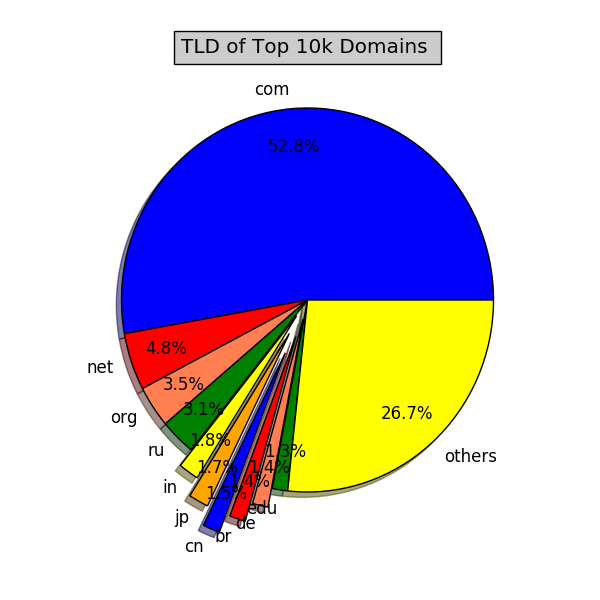
\includegraphics[height=8cm,width=8cm]{images/figure/figure_2.png}
% \end{figure}




  \begin{frame}{HTTPS证书服务商}
    % HTTPS 测试整体情况:
    % \begin{columns}
    %   \begin{column}{0.5\textwidth}
    %     \begin{table}
    %       \tiny
    %     \begin{tabular}{r|l|l|l|l}
    %       \toprule
    %               & Total & Succeeded & Failed &  Refused \\
    %       \midrule
    %       (domain, ip) & 47877& 25740 & 1245 &1028\\
    %       domain name&   8585&5376& 755 &753\\
    %       \bottomrule
    %       \end{tabular}
    %     \end{table}
    %   \end{column}
    %   \begin{column}{0.5\textwidth}
    %     \begin{figure}
    %       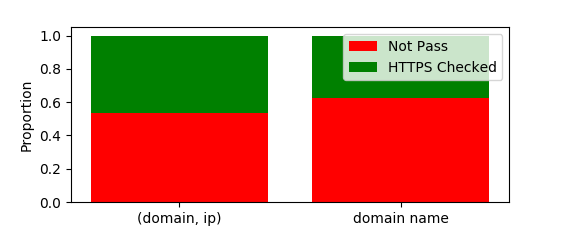
\includegraphics[height=2cm]{images/figure/figure_httpscheck.png}
    %       \end{figure}
    %   \end{column}
    %   \end{columns}
HTTPS 证书服务商统计:
\begin{columns}
      
  \begin{column}{0.5\textwidth}
    \begin{table}
      \tiny
    \begin{tabular}{r|l|l}
      \toprule
      Service Provider &Quantity & Percent\\
      \midrule
      COMODO CA Limited&2006 & 37.22\%\\
      DigiCert Inc&1041& 19.31\%\\
      GlobalSign &393& 7.29\%\\
      GoDaddy.com, Inc.&334& 6.19\%\\
      GeoTrust Inc.&281& 5.21\%\\
      Symantec Corporation&197& 3.65\%\\
      Amazon&190& 3.53\%\\
      CloudFlare, Inc.&157& 2.91\%\\
      Google Trust Services&148& 2.75\%\\
      Others & 643& 11.93\%\\
      \bottomrule
      \end{tabular}
    \end{table}


  \end{column}
  \begin{column}{0.5\textwidth}
    \begin{figure}
      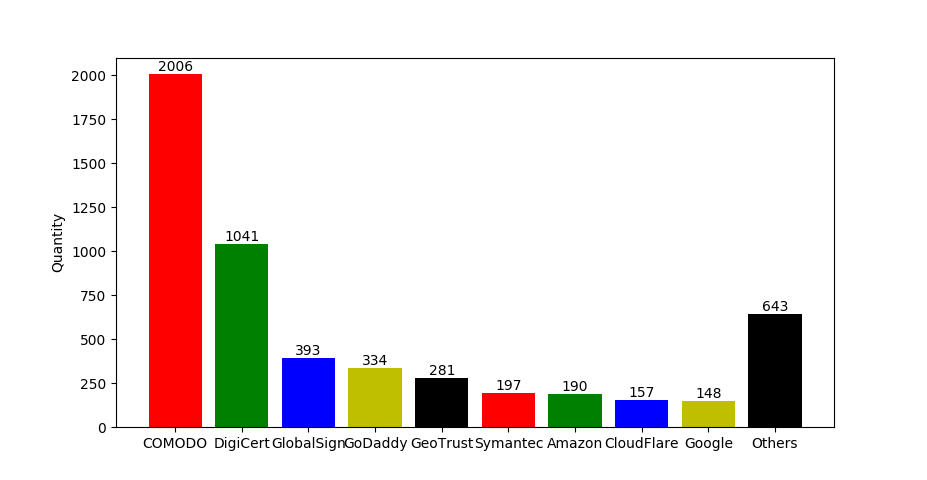
\includegraphics[height=3.5cm]{images/figure/certserver.png}
      \end{figure}
  \end{column}
  \end{columns}

  对cn顶级域名下证书服务商进行考察,情况与上表类似。

    
  \end{frame}

  

  \subsection{对开放解析器的考察}
  \begin{frame}{开放解析器}
    对ZMap检测到的1.6万个解析器进行数据分析:
    \begin{columns}
      
      \begin{column}{0.5\textwidth}
        \begin{table}
          \tiny
          \begin{tabular}{r l l l}
            \toprule
            countryName &counts & DNSSEC & Percent\\
            \midrule
                 
            United States &	2028 &266&13.12\%\\
            Republic of Korea &	2022&60&2.97\%\\
            Taiwan &	1098&41&3.73\%\\
            Russia &	1087&90&8.28\%\\
            Indonesia &	806&27&3.35\%\\
            Japan &	638&30&4.70\%\\
            United Kingdom &	529&35&6.62\%\\
            Poland &	462&30&6.49\%\\
            France &	450&52&11.56\%\\
            Brazil &	438& 61&13.93\%\\
            \bottomrule
            \end{tabular}
        \end{table}
    
      \end{column}
      \begin{column}{0.5\textwidth}
        \begin{figure}
          \centering
          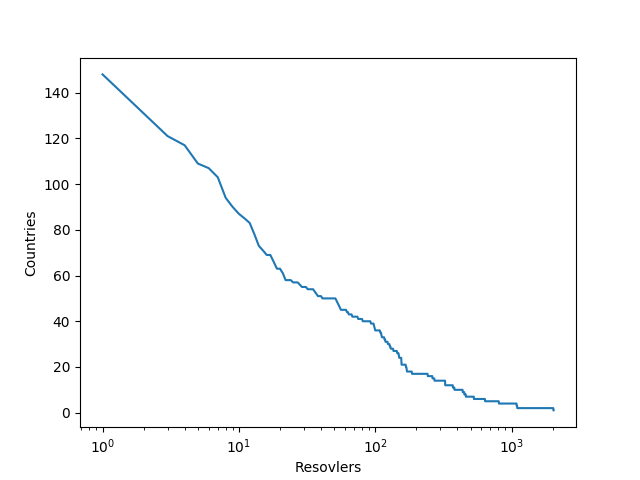
\includegraphics[height=4cm]{figures/resolvercy.png}
          % \caption{各个国家检测到解析器的数量}
          \label{fig:resolvercy}
        \end{figure}
      \end{column}
      \end{columns}
  
  \end{frame}



\begin{frame}{解析正确性判断}
\begin{itemize}
  \item 1373个域名在16488个解析器上进行查询,最终获得926万个(domain, res, ip)三元组,16万(domain, ip)二元组
  \item 右图为联合分析算法的\texttt{IPTrust}结果与HTTPS验证结果进行对照的图像
  \item 一些国家的解析器会使用某些特殊IP地址作为对很多不相干域名的查询的响应,如左边表格所示

\end{itemize}

  \begin{columns}
      
    \begin{column}{0.5\textwidth}
      \begin{table}
        \tiny
        \begin{tabular}{r l l l}
          \toprule
          Country &IP & Counts & Domain Example\\
          \midrule
               
          IRAN &	10.10.34.34&131&bilibili.com\\
          UAE &	10.10.34.35&32&sex.com\\
          FINLAND &	0.0.0.0 & 27 &exosrv.com\\
          PORTUGAL &	0.0.0.0&19&badoo.com\\
          ROMANIA &	0.0.0.0&11&cnzz.com\\
          LATVIA &	0.0.0.0&11&duba.com\\
          SERBIA &	79.101.14.184&7&www.goal.com\\
          B\&H &	127.42.0.0& 7&hatenablog.com\\
          CYPRUS &	127.42.0.0&6&iqoption.com\\
          DENMARK &	80.239.178.184&5&hm.com\\
          \bottomrule
          \end{tabular}
      \end{table}
  
    \end{column}
    \begin{column}{0.5\textwidth}
      \begin{figure}
        \centering
        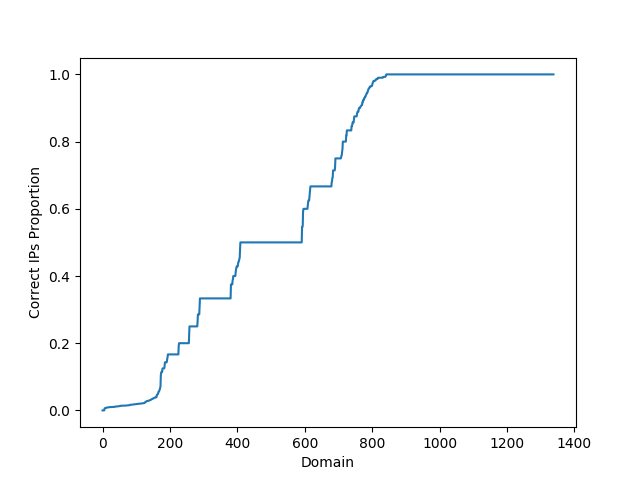
\includegraphics[height=4cm]{figures/tlsvsal.png}
        % \caption{各个国家检测到解析器的数量}
        \label{fig:resolvercy}
      \end{figure}
    \end{column}
    \end{columns}
\end{frame}

\begin{frame}{CDN 识别判断}
  \begin{itemize}
    \item 使用联合分析算法经过迭代得到\texttt{DomainSimilarity} 矩阵
    \item 查找其中的连通分量,一个连通分量代表一个CDN的集群,最大的CDN集群的统计如下表所示
    \item 我们得到了数百个集群,通过验证对应组织名称的相似性对CDN识别算法进行验证,结果如右图
  \end{itemize}
  \begin{columns}
      
    \begin{column}{0.5\textwidth}
      \begin{table}
        \tiny
        \begin{tabular}{r l l}
          \toprule
          CDN &Size &Domain\\
          \midrule	
         Google &	119 & google.com \\
         Fastly & 73 & airbnb.com \\
         Amazon  &	40 & time.com\\
         Akamai & 20 & ebay.com \\
         CloudFlare & 10 & 4chan.org \\
         AliCloud & 7 & tmall.com \\
         Verizon & 6 & bing.com \\
         Incapsula & 6 & prothomalo.com \\
          \bottomrule
          \end{tabular}
      \end{table}
  
    \end{column}
    \begin{column}{0.5\textwidth}
      \begin{figure}
        \centering
        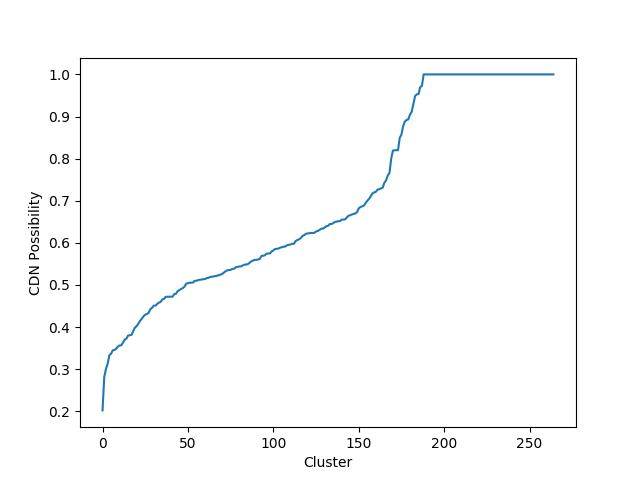
\includegraphics[height=4cm]{figures/cluster.png}
        % \caption{各个国家检测到解析器的数量}
        \label{fig:resolvercy}
      \end{figure}
    \end{column}
    \end{columns}
\end{frame}
 \begin{frame}{参考文献}
  \tiny
  \bibliographystyle{unsrt}%Used BibTeX style is unsrt
  \bibliography{ref}
\end{frame}

\begin{frame}
  \begin{figure}
    
\includegraphics[height=2.23cm,width=4.29cm]{images/thank.jpg}
  \end{figure} 
\end{frame}
\end{document}

